\documentclass[12pt]{article}
\usepackage{amsmath, amsfonts, amsthm, amssymb, latexsym, enumerate}
\oddsidemargin=0in \topmargin=-.5in \textwidth=6.75in \textheight=9.25in
\usepackage[utf8]{inputenc}
\usepackage{tikz}
\usepackage{recycle}
\usepackage{hyperref}
\usepackage{algorithm}
\usepackage[noend]{algpseudocode}
\usepackage{amsmath}
\usepackage{mathtools}
\usepackage{pdfpages}
\DeclarePairedDelimiter\ceil{\lceil}{\rceil}
\DeclarePairedDelimiter\floor{\lfloor}{\rfloor}

\usepackage{mdframed}
\newmdtheoremenv{theo}{Theorem}

\def\ints{{\mathbb Z}}
\def\rats{{\mathbb Q}}
\def\nats{{\mathbb N}}
\def\reals{{\mathbb R}}
\def\complex{{\mathbb C}}
\def\quats{{\mathbb H}}
\def\proj{{\mathbb P}}
\def\aff{{\mathbb A}}
\def\FF{{\mathbb F}}
\def\Gp{{\mathbb G}}
\def\adeles{{\mathbb A}}
\def\Ab{{\mathfrak Ab}}
\def\Hecke{{\cal H}}
\def\Fourier{{\cal F}}
\def\one{{\bf 1}}
\def\diag{{\bf diag}}
\def\del{{\partial}}
\def\Span{{\textsc Span}}
\def\qed{\hfill $\Box$}
\def\Im{{\text{Im }}}
\def\im{{\text{im }}}
\def\lcm{{\text{lcm }}}
\def\rank{{\text{rank }}}
\def\sech{{\text{sech }}}
\def\csch{{\text{csch }}}
\def\st{{\text{ s.t. }}} 
\def\nullity{{\text{nullity }}}
\def\Re{{\text{Re}}}
\def\Hom{{\text{Hom}}}
\def\sheafhom{\mathcal{H}om}
\def\Tor{{\text{Tor}}}
\def\cd{{\text{cd }}}
\def\ord{{\text{ord}}}
\def\trace{{\text{tr }}}
\DeclareMathOperator{\eff}{eff}
\def\res{{\text{res}}}
\def\Proj{{\text{Proj }}}
\def\Hess{{\text{Hess }}}
\def\grad{{\text{grad }}}
\def\cf{{\text{char}}}
\def\Frac{{\text{Frac}}}
\def\codim{{\text{codim }}}
\def\coker{{\text{coker }}}
\def\height{{\text{ht }}}
\def\Ext{{\text{Ext}}}
\def\trdeg{{\text{tr.deg. }}}
\def\cis{{\text{cis }}}
\def\Cl{{\text{Cl }}}
\def\Div{{\text{Div }}}
%\def\Aut{{\text{Aut}}}
\DeclareMathOperator{\Aut}{Aut}
\def\Out{{\text{Out}}}
\def\Gal{{\text{Gal}}}
\def\Ind{{\text{Ind}}}
\def\mod{{\mbox{mod }}}
\def\supp{{\mbox{supp }}}
\def\Ann{{\mbox{Ann }}}
\def\Spec{{\mbox{Spec }}}
\def\Specbf{{\textbf{Spec }}}
\def\Pic{{\text{Pic }}}
\def\Max{{\mbox{Max }}}
\def\mc#1{\mathcal{#1}}
\def\mf#1{\mathfrak{#1}}
\def\ol#1{\overline{#1}}
\def\ul#1{\underline{#1}}
\def\v#1{\vec{#1}}
\def\ideles#1{{\mathbb A^{\times}_{#1}}}
\def\pairing#1#2{\langle #1, #2 \rangle}
\def\legendre#1#2{\left( \frac{#1}{#2} \right)}

\def\mapright#1{\smash{\mathop{\longrightarrow}\limits^{#1}}}
\def\mapdown#1{\Big\downarrow \rlap{$\vcenter{\hbox{$\scriptstyle#1$}}$}}

\def\matrix#1#2#3#4{
    \left( \begin{array}{cc} #1&#2 \\ #3&#4 \end{array} \right)}
\def\threematrix#1#2#3#4#5#6#7#8#9{
    \left( \begin{array}{ccc} #1&#2&#3 \\ #4&#5&#6 \\ #7&#8&#9 \end{array} \right)}
\def\columnvector#1#2{
    \left ( \begin{array}{c} #1 \\ #2 \end{array} \right)}
\def\columnthreevector#1#2#3{
    \left ( \begin{array}{c} #1 \\ #2 \\ #3 \end{array} \right)}
\def\rowvector#1#2{
    \left ( \begin{array}{cc} #1 & #2 \end{array} \right)}
\def\rowthreevector#1#2#3{
    \left ( \begin{array}{ccc} #1 & #2 & #3 \end{array} \right)}
\def\blockmatrix#1#2#3#4{
    \left( \begin{array}{c|c} #1 & #2 \\ \hline #3 &
    #4 \end{array} \right)}
\def\Lie#1{{\mathfrak #1}}

\def\iff{\Longleftrightarrow}

\def\transpose {{\sp t}}
\def\half{{1 \over 2}}

\newtheorem{theorem}{Theorem}[section]
\newtheorem{prop}[theorem]{Proposition}
\newtheorem{lemma}[theorem]{Lemma}
\newtheorem{corollary}[theorem]{Corollary}
\newtheorem{predefinition}[theorem]{Definition}
\newenvironment{definition}{\begin{predefinition}\rm}{\end{predefinition}}
\newtheorem{preremark}[theorem]{Remark}
\newenvironment{remark}{\begin{preremark}\rm}{\end{preremark}}
\newtheorem{preconstruction}[theorem]{Construction}
\newenvironment{construction}{\begin{preconstruction}\rm}{\end{preconstruction}}
\newtheorem{prenotation}[theorem]{Notation}
\newenvironment{notation}{\begin{prenotation}\rm}{\end{prenotation}}
\newtheorem{preexample}[theorem]{Example}
\newenvironment{example}{\begin{preexample}\rm}{\end{preexample}}
\newtheorem{preclaim}[theorem]{Claim}
\newenvironment{claim}{\begin{preclaim}\rm}{\end{preclaim}}
\newtheorem{prequestion}[theorem]{Question}
\newenvironment{question}{\begin{prequestion}\rm}{\end{prequestion}}

%\newcommand {\thmref}[1] {Theorem \ref{#1}}                                                  
%\newcommand {\lemmaref}[1] {Lemma \ref{#1}}                                                  
%\newcommand {\propref}[1] {Proposition \ref{#1}}                                             
%\newcommand {\remref}[1] {Remark \ref{#1}}                                                   
%\newcommand {\conjref}[1] {Conjecture \ref{#1}}                                              
%\newcommand {\claimref}[1] {Claim \ref{#1}}                                                  
%\newcommand {\defnref}[1] {Definition \ref{#1}}                                              
%\newcommand {\corref}[1] {Corollary \ref{#1}}                                                
%\newcommand {\caseref}[1] {Case \ref{#1}}                                                    
%\newcommand {\exref}[1] {Example \ref{#1}}                                                   
%\newcommand {\exsref}[1] {Examples \ref{#1}}                                                 
%\newcommand {\eqnref}[1] {Equation \ref{#1}}

\newcommand{\bbmu}{\mu\hspace{-0.065in}\mu}
\newcommand{\bbalpha}{\alpha\hspace{-0.065in}\alpha} 

%%%%%%%%%%%%%%%%%%%%%%%%%%%%%%%%%%%%%%%%%%%%%%%%%%%%%%%%%%


\documentclass{article}
\usepackage[utf8]{inputenc}

\title{Detecting Gerrymandering with Probability: A Markov Chain Monte Carlo Model}
\author{Jackson Barkstrom, Rohan Dalvi, Christopher Wolfram}
\date{November 11, 2018}

\begin{document}

\begin{titlepage}
\maketitle
\end{titlepage}


\tableofcontents
\pagebreak

\section{Nontechnical Summary}
%    Gerrymandering--the drawing of electoral districts in order to favor one political group--can dramatically bias the outcomes of elections. However, although some constraints exist against it, Gerrymandering largely goes unchecked in the United States because no judicially manageable standard exists to prevent it. No one seems to agree on a way to define it! Recently, a metric known as the efficiency gap that measures wasted votes by party was introduced as a simple, one-size-fits all approach to quantify Gerrymandering. However, although useful and highly correlated with Gerrymandering, we explain the metric and many of its shortcomings near the end of our paper.
%    \par
%    Rather than invent another metric like the efficiency gap, which will have its inherent flaws and difficulties standing up in a court of law, we present a commonsense method to systematically detect and quantify instances of Gerrymandering with probability. 
%    Essentially, we randomly generate possible district drawing schemes to determine whether or not the current districting scheme is extremely biased. If the current districting scheme just so ``happens'' to elect more members of one party than 99.99\% of all possible districting schemes (which we will approximate with a random sample), I think we can safely say it is the result of party-driven Gerrymandering!
%    \par
%    Actually generating ``random'' ... (talking about challenges)
%    \par
%    In using our method, we first quantify the extent of Gerrymandering in North Squarolina, a hypothetical square-shaped state. Next, we generalize our model to any hypothetical districting scheme and apply it to the state of North Carolina. 
    
    Gerrymandering--the drawing of electoral districts in order to favor one political group--can dramatically bias the outcomes of elections. However, it is difficult to combat Gerrymandering because it is hard to quantify. Recently, a metric known as the efficiency gap has come to prominence as a simple formula for measuring Gerrymandering by looking at wasted votes (votes that did not affect the outcome of an election). The efficiency gap formula, however, has a number of issues. These are explored more in section 6, but essentially efficiency gap measures more than just Gerrymandering.
    \par We propose another, statistical approach. We compare the properties of random districtings to proposed districtings to see if the proposed districts would lead to a significantly different election outcome. That is, our random districtings give us a baseline with which we can compare proposals, and we can see if the proposals have been designed to land at the far tails of the distribution, optimizing for one party or the other.
    \par We start with simple random districtings, but we add more and more sophistication until we can generate valid random districtings for not just North Squarolina, but also arbitrary real-world states.
    \par We find that proposed districting (C) produces an extremely unlikely election outcome, suggesting that it is Gerrymandered.

\section{Introduction}
    Our job is to detect the occurrences of Gerrymandering. According to the Cornell Legal Information Institute, Gerrymandering describes ``when political or electoral districts are drawn with the purpose of giving one political group an advantage over another, a practice which often results in districts with bizarre or strange shapes'' \cite{CLLI}. Historical evidence shows that the presence of Gerrymandering can significantly change outcomes of public policy \cite{psmag}. Currently three main constraints exist in the United States prohibiting Gerrymandering \cite{problem}, namely: 
    \begin{enumerate}
    \item \textbf{Contiguity.} Every voting district must have a connected interior whenever possible.
    \item \textbf{One Person, One Vote.} Voting districts must contain populations of nearly equal size.
    \item \textbf{Voting Rights Act.} Voting districts must not dilute the votes of protected minorities.
    \end{enumerate}

    Despite these constraints, what most people might think of as partisan Gerrymandering often occurs in the U.S. because there is no judicially managable standard to enforce ``fair'' partisan districting. The Supreme Court has indicated that extreme partisan Gerrymandering--districting that dramatically favors one party over the other--is unconstitutional \cite{GW}, but courts have no method to even define extreme partisan Gerrymandering. Recently in the case \textit{Gill v. Whitford} (2018), a metric known as efficiency gap that measures ``wasted votes'' by party was used to try to prove unfair districting in Wisconsin. Efficiency gap generally correlates with Gerrymandering. In a hypothetical unfair districting scheme using four districts of equal size, for example, a party that has 60\% of the popular vote might only win a quarter of all district elections. The majority party will have ``wasted'' nearly all of its votes by barely losing three elections and winning one in a landslide. In the losing cases, every vote is wasted, and in the landslide case all but the votes needed to win are wasted. Since one party wasted nearly all of its votes and the other party wasted almost none, the efficiency gap metric for this election will be extremely high. And obviously, this could easily be a Gerrymandered election: a party with 60\% majority won only 25\% of the districts! However, although this obvious example shows the success of the efficiency gap, the efficiency gap is absolutely not a reliable, one-size-fits all method to detect Gerrymandering. During \textit{Gill v. Whitford} the reliability of the metric itself was called into question, and a high efficiency gap was not accepted by the Supreme Court as proof of Gerrymandering in Wisconsin. Later in the paper, we will look more at the efficiency gap and explain some of its flaws.
    \subsection{Our Method}
    Our method, unlike the efficiency gap, is not a metric. It is a method based on the simple idea of probability. We try to produce a randomly generated sample of all reasonable districtings--a sample of all ways to reasonably draw district boundaries--and we use the sample to test for Gerrymandering. If we are able to produce a sample that approximates well enough a random sample, we can use this generated sample to test for unfair districting. We can mostly figure out if a certain arrangement is Gerrymandered by comparing it with a random sample all possible district arrangements. If the arrangement we are testing elects more members of one party than almost any other arrangement randomly generated, if it is abnormal enough, we can say that it is probably Gerrymandered. Statistically, if the chances of randomly producing a district that happens to favor one party by at least a certain amount is .001, we can be almost certain that the district was Gerrymandered.
    \par
    True random generation of a sample of reasonable districtings is almost impossible to achieve--the computational power required to generate a random sample of contiguous districts is absurdly large as the size of our space increases. This is because most randomly generated district mappings are not contiguous--thus if $1$ in $10000$, $10000000$, \frenchspacing etc. \nonfrenchspacing of our randomly generated district mappings are contiguous our generation will take a very, very long time. Thus, instead of a truly random model, we use a Markov Chain Monte Carlo method to approximate random contiguous districting samples of equal size (or at least as equal as possible). We start with $n$ districts, and we randomly change out pieces of each district with pieces of other districts as the districts appear to walk around each other when visualized. We do this many, many times and then take all the districts that the chain generated as our random sampling of all possible electoral district drawings. The strength of this approach, as we will show later, is that as the number of steps in the Markov Chain increases our sampling gets closer and closer to a random sample of all contiguous districts of the same size. Of course there will always be some bias in our chain based on the initial condition. This approach was introduced in 2014 by Fifield, Higgins, Imai, and Tarr \cite{Harv}. However, their approach uses geographical compactness and other subjective factors. Our approach is far simpler because the only constraints on our model are the objective factors of equal size and contiguity. 
    
%%\subsection{The Impact of Gerrymandering}
  %%  Include the graphs chris made about what Gerrymandering can do at its worst. Model on the sigmoid and look at outliers. Maybe try to get this specifically applied to squarolina?
  
  
\subsection{North Squarolina}
    We have been tasked with evaluating the redistricting proposals of a hypothetical state, North Squarolina. North Squarolina consists of 36 voting blocks, arranged in a $6$x$6$ grid, with each voting block containing the same number of voting citizens and consistently voting unanimously for the same party. The voting behavior is illustrated in (V). Because of this consistent behavior, we can assume that Gerrymandering is possible: one must be able to predict voting behavior in order to Gerrymander. We have been asked to evaluate three different redistricting proposals labeled (A), (B) and (C) below. We investigate in the results section of this paper if any of them appear to be Gerrymandered in favor of either Redublicans or Bluemocrats. Henceforth, we refer to Redublicans as "Red" and Bluemocrats as "Blue".
    
    \begin{figure}[h!]
    \centering
    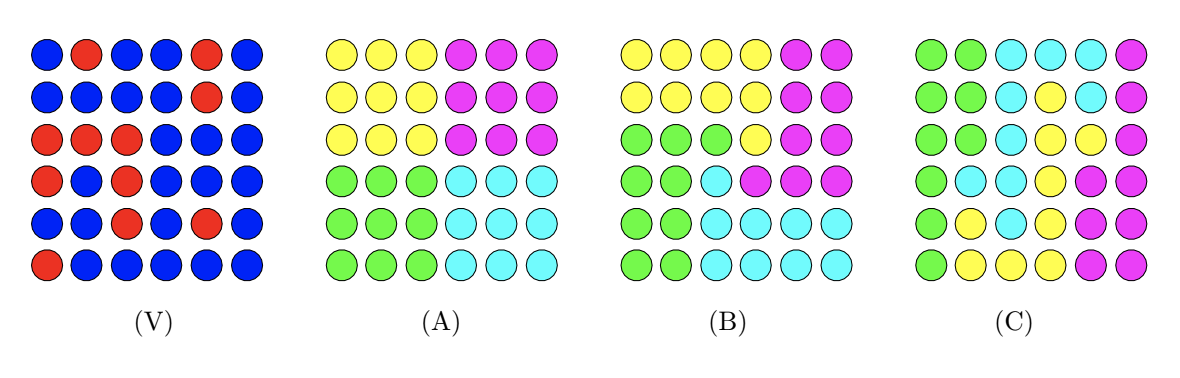
\includegraphics[scale=0.8]{squarolina}
    \label{fig:squarolina}
    \end{figure}
\subsection{What About North Carolina?}
Later in the paper we will also apply our method to the real state of North Carolina to see whether or not it was gerrymandered, based on past data.





\section{Model}
    \subsection{Model Introduction}
    The goal of our model is to produce a large number (on the order of hundreds of thousands) of districtings, as randomly as possible, in order to obtain a highly representative sample of the space of all possible districts. By examining this very large sample, we can determine the probability of a given districting's voting outcome in the space of all voting outcomes for a particular voting arrangement. In other words, we can determine the probability of a given party winning \(x\) seats based on the arrangement of voting blocks. If a particular districting is a statistically significant outlier and produces voting outcome with a low probability, then the districting is likely biased. In the case of North Squarolina, if a districting scheme just so happens – with a .00000001\% chance – to elect more Redublicans than almost any other districting scheme, we can safely say that the district is Gerrymandered! 
    \par
    We begin by developing a basic model of random district generation and then improve iteratively. Our first iteration relies on random selection of voting blocks into districts in order to generate districts. Our second iteration of the model accounts for the fact that districts are legally required to contain the same number of voters. Our third iteration ensures that the contiguity of districts is preserved through the use of a Markov Chain Monte Carlo (MCMC) random walk. We demonstrate that the districtings obtained via the Markov Chain closely approximate randomly generated districtings.
    All algorithms implemented in Mathematica.
    \par
    \subsubsection{Mathematical Definitions}
    Here we formally define the terms we use in the rest of the paper. We represent a given voter arrangement as an \(m \times n\) matrix \(V\) (computationally, this is an array). Each entry in \(V\) represents a voting block. V is populated by values describing the difference between votes for party A and votes for party B in historical voting data. We represent districting \(D\) as an \(m \times n\) matrix. Each districting includes \(g\) districts . Each entry in \(D\) represents a voting block, like in A, so both arrays describe the same geography. Each entry in \(D\) consists of a value taken from the list of all "grouping value" \(L=\{l_1, l_2...l_g\}\), where each grouping value \(l_i\) corresponds to a different district. There are \(g\) districts, and each district is a set of entries in \(D\) with the same value.  The voting outcome \(V\) is obtained by summing all entries in $V$ corresponding to a district in \(D\). For each district, if the sum of entries is greater than 0, then Party A won the seat. If it is less than 0, then Party B won the seat. This procedure can be performed across all districts to obtain a total number of seats won for Party and Party B respectively. \(V\) and \(D\) can also be treated as graphs, and the same logic that applies above still functions by replacing the word "entries" of \(V\) and \(D\) with "nodes" of \(V\) and \(D\).
    \par
    In the case of North Squarolina, the outcome of voting in any voting block is assumed to be unanimous and to have equal populations. Hence, all entries in \(V\) can be normalized and are equal to either either -1 or 1.
\subsection{Random Districts}
    The first method we develop is random generation of districtings. In this method we assign each voting block to a random district. Mathematically, this means that each entry in D (representing a particular voting block) is randomly assigned a grouping value, as shown in Algorithm \ref{alg:rd}. The value assigned to a given voting block is random. We term this district-generation algorithm the "Random Districts" (RD) Algorithm. Note that functions not defined here are pre-defined in Mathematica, the scientific computing language we used, or are implemented trivially. Implementation of this algorithm (and all other algorithms mentioned) are in the code appendix. 
    
\begin{algorithm}
\caption{Random Districts algorithm}\label{alg:rd}
\begin{algorithmic}[]
\Procedure{RD}{$V$}
\State{$D\gets0$}\Comment{$0$ is zero matrix}
\State{$O\gets\emptyset$}\Comment{$O$ is the set of voter outcomes}
\For{$d_i_,_j \in D$}
    \State $d_i_,_j \gets rand(L)$ \Comment{Randomly assigns values from L}
\EndFor
\For{$l_i \in L$}
    \State{$O \gets O \cup outcomes(l_i, V)$}\Comment{counts voting outcomes for each state}
\EndFor
\EndProcedure
\end{algorithmic}
\end{algorithm}

    The $outcomes$ function determines the voting outcome for a district whose voting blocks have grouping value $l_i$ through the method outlined in the mathematical definitions section. The result is that the set of all outcomes $O$ obtains a list of each voting outcome given a specific voter arrangement.

\subsection{Random Districts of Equal Size}
An issue with the randomly generated districts obtained via Algorithm \ref{alg:rd} is that they are not all the same size. Based off of the assumption that each voting block has equal population, then it is possible that districtings will be generated where each district has a different number of voting blocks. The votes of of people in districts with fewer voting blocks will therefore "count more" as these individuals have more power in selecting which party wins the seat in their district than individuals in a district where there are more voting blocks. Consequently, we modify the RD algorithm to generate random districts of \textit{equal size}. This is shown in algorithm \ref{alg:esrd}. We term this algorithm the Equal-Size Random District (ESRD) algorithm.

\begin{algorithm}
\caption{Equal-Size Random Districts algorithm}\label{alg:esrd}
\begin{algorithmic}[]
\Procedure{ESRD}{$V$}
\State{$D\gets0$}
\State{$O\gets\emptyset$}
\State $\{D_1, D_2...D_g\} \gets partition(D)$ \Comment{randomly partitions entries of \(D\) into \(g\) 1-D arrays}
\For{$D_i \in \{D_1, D_2...D_g\}$}
    \For{$v_i \in D_i$}\Comment{\(v_i\) is an entry in D corresponding to a voting block}
        \State{$v_i=l_1$}
        \State $V\getsV$\Comment{}
    \EndFor
\EndFor
\For{$l_i \in L$}
    \State{$O \gets O \cup outcomes(l_i)$}\Comment{counts voting outcomes for each state}
\EndFor
\EndProcedure
\end{algorithmic}
\end{algorithm}

The fundamental flaw in the ESRD algorithm is that it is not able to intentionally generate contiguous districts. Though consistent sizes, the districts generated through this algorithm are spatially random. Therefore, voting blocks in the same district will likely be disconnected from each other. One solution to this is to repeatedly generate districtings with the ESRD algorithm until a districting with contiguous districts is obtained. But this is highly computationally inefficient. Evidence of this inefficiency is included in the code appendix.
\subsection{Contiguous Districts with Markov Chain Monte Carlo}
In order to generate a near-random distribution of districtings, we use a Markov Chain Monte Carlo (MCMC) algorithm. However, in the random walk, we limit possible changes in the districting to ones that preserve contiguity. Using \(n\) iterations and taking an initial contiguous districting \(D_0\) represented as a graph, we produce the following:

\begin{algorithm}
\caption{MCMC algorithm}\label{alg:mcmc}
\begin{algorithmic}[]
\Procedure{ESRD}{$D_0, V$}
\State{$O\gets\emptyset$}
\For{$l_i \in L$} \Comment{Obtain districts from the districting}
        \State $D_i \gets {d_i \in D_0 : d_i= l_i}$
\EndFor
\While{$i<n$}
    \State{$s \gets sizemin({D_1...D_g})$}\Comment{Sets \(s\) to be one of the smallest districts}
    \State{$r \gets random\_neighbor(s)$}
    \If{$(is\_connected(remove(s, r)$))}\Comment{if removing \(r\) preserves contigruity}
    \State{$a \gets size(s)$)}
    \State{s \gets \{s_1,... ,s_n, r\}}\Comment{move \(r\) into \(s\)}
    \EndIf
    \State{$i \gets i+1$}
    \State{remove(s, r)}
    \For{$l_i \in L$}
        \State{$O \gets O \cup outcomes(l_i)$}\Comment{counts voting outcomes for each state}
    \EndFor
\EndWhile
\EndProcedure
\end{algorithmic}
\end{algorithm}
In the algorithm above, we choose the smallest districts (randomly choose if there are multiple smallest districts) and then randomly give it another voting block that touches it, on the terms that taking the block won't violate contiguity of another region. $random\_neighbor$ obtains a random voting block adjacent to \(s\). Also, $remove(r, s)$ removes the voting block $r$ from $s \in D$. Additionally, $is\_connected$ checks if a given graph is connected.

In reality, the MCMC is not truly random. The initial "seed" districting will bias districtings obtained from higher iterations towards the original position. This is reflected in the dependence of the algorithm on $D_0$. However, by increasing the count of iterations, the result is that the Markov Chain is nearly random. This issue is explored more below.

\subsubsection{Approximation of Randomness}
    Figure \ref{fig:convergence} depicts the state of the Markov chain at increasingly high values of \(i\) in the algorithm \ref{alg:mcmc}. The figure depicts the frequency that voting blocks were assigned to a specific district (i.e., the frequency with which they had a certain grouping value) in a single run of the Markov Chain. Black is O (never passed over), white is 1 (always passed over), and grey is somewhere in the middle. If we see that over time the frequency of each voter block in the Markov Chain becomes roughly equal, then this means that each voter block has been assigned to the specified district ("passed over by the Markov Chain") a roughly equal number of times. A truly random sample would have the same property--a truly random sample would be the same shade of grey in all squares--and this is the key property of randomness that our Markov Chain can approximate.
    
    \begin{figure}[h!]
    \centering
    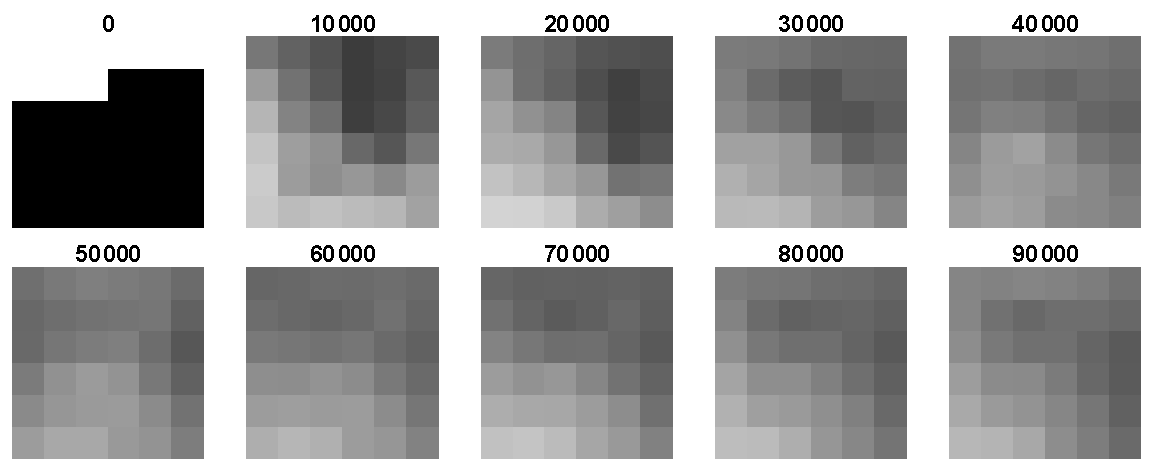
\includegraphics[scale=0.9]{convergence}
    \caption{MCMC Convergence - 100,000 Runs}
    \label{fig:convergence}
    \end{figure}    
    
    \par
    As shown in the $i=0$ case, one district begins in the top left, as the Markov chain has not begun yet. We can see in the $i=10,000$ case, we obtain a visibly biased distribution of frequency with which the Markov chain has passed over different voting blocks, with blocks in the upper right being significantly more likely to be passed over. However, by the $i=90,000$ case, the amount that each voting block has been passed over by the chain has gotten much more even. This suggests that our $100000$ iterations is enough to ensure that our districts are effectively random, and that the initial condition will not have too strong an effect.

\subsubsection{Random Seeding to for A Better Approximation}
    Further improvement in the pseudo-random behavior of the Markov Chain can be obtained by seeding the initial position of the chain randomly. Doing this is equivalent to the procedure described above, except the first $n$ voter outcomes are not recorded. See the Code Appendix for further details.
%\subsection{Random Voter Arrangements}
%How we generate random arrangements of voters
%Used to obtain the graph comparing average number of seats won vs. number of voters for a party

\subsubsection{More Random Seeding to for An Even Better Approximation}
    To seed our MCMC algorithm, we just need to give it any districting where all districts are contiguous. By repeatedly applying MCMC, any deviations in the sizes of the districts will be evened out. However, if we generate a seed graph with districts of wildly different sizes, it will take longer for it to converge on an equal-area districting.
    \par We developed an algorithm for getting around this. We take the graph that we used to represent the adjacency of voting blocks (a grid graph in the case of North Squarolina), we remove all of the edges, and then we repeatedly add edges back to the smallest connected component until we have the desired number of connected components (see Code Appendix for details). This leaves us with a districts of similar size that can be fed to MCMC.

\section{Results}
\subsection{Do Any of the Proposals Gerrymander North Squarolina?}
We look at the number of districts that will be won by red under each districting proposal. If this number is abnormally low, we might find evidence of a blue-driven Gerrymander, and if the number is abnormally high, we might find evidence of a red-driven Gerrymander.
Assuming that voting patterns stay the same in North Squarolina, like they have in the past, red will win 0 districts under (A), 1 district under (B), and 2 districts under (C).
\begin{figure}[h!]
\centering
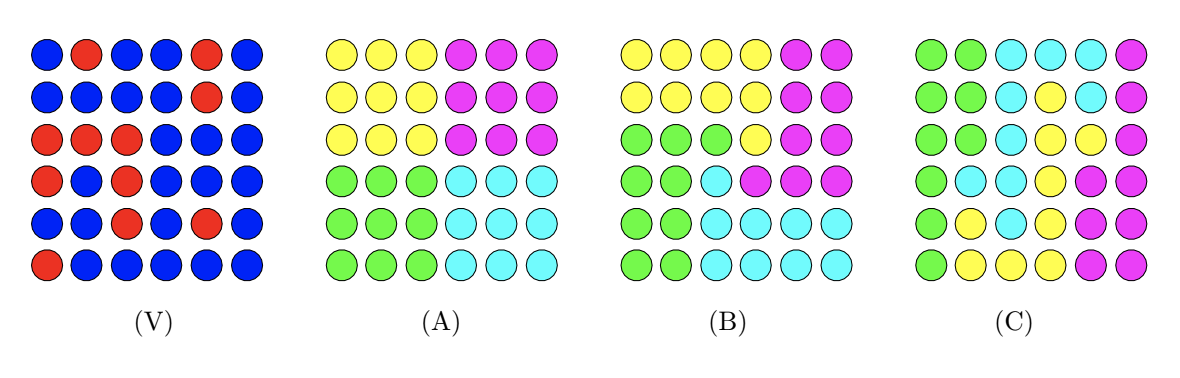
\includegraphics[scale=0.8]{squarolina}
\label{fig:squarolina}
\end{figure}
\subsubsection{Using Random Districts}
Our Random Districts algorithm is not terribly accurate because it allows for districts that are wildly different sizes. An example districting obtained by the RD algorithm is shown below (Figure \ref{fig:rdd}).

    \begin{figure}[h!]
    \centering
    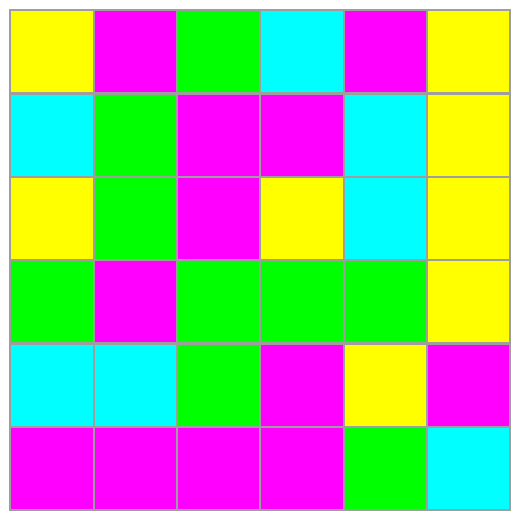
\includegraphics[scale=0.60]{rd_districting.pdf}
    \caption{North Squarolina, Random Districts Histogram}
    \label{fig:rdd}
    \end{figure}

It also allows for non-contiguous districts. In fact, when we generated 100000 completely random districtings, none of them contained only contiguous districts.
    \begin{figure}[h!]
    \centering
    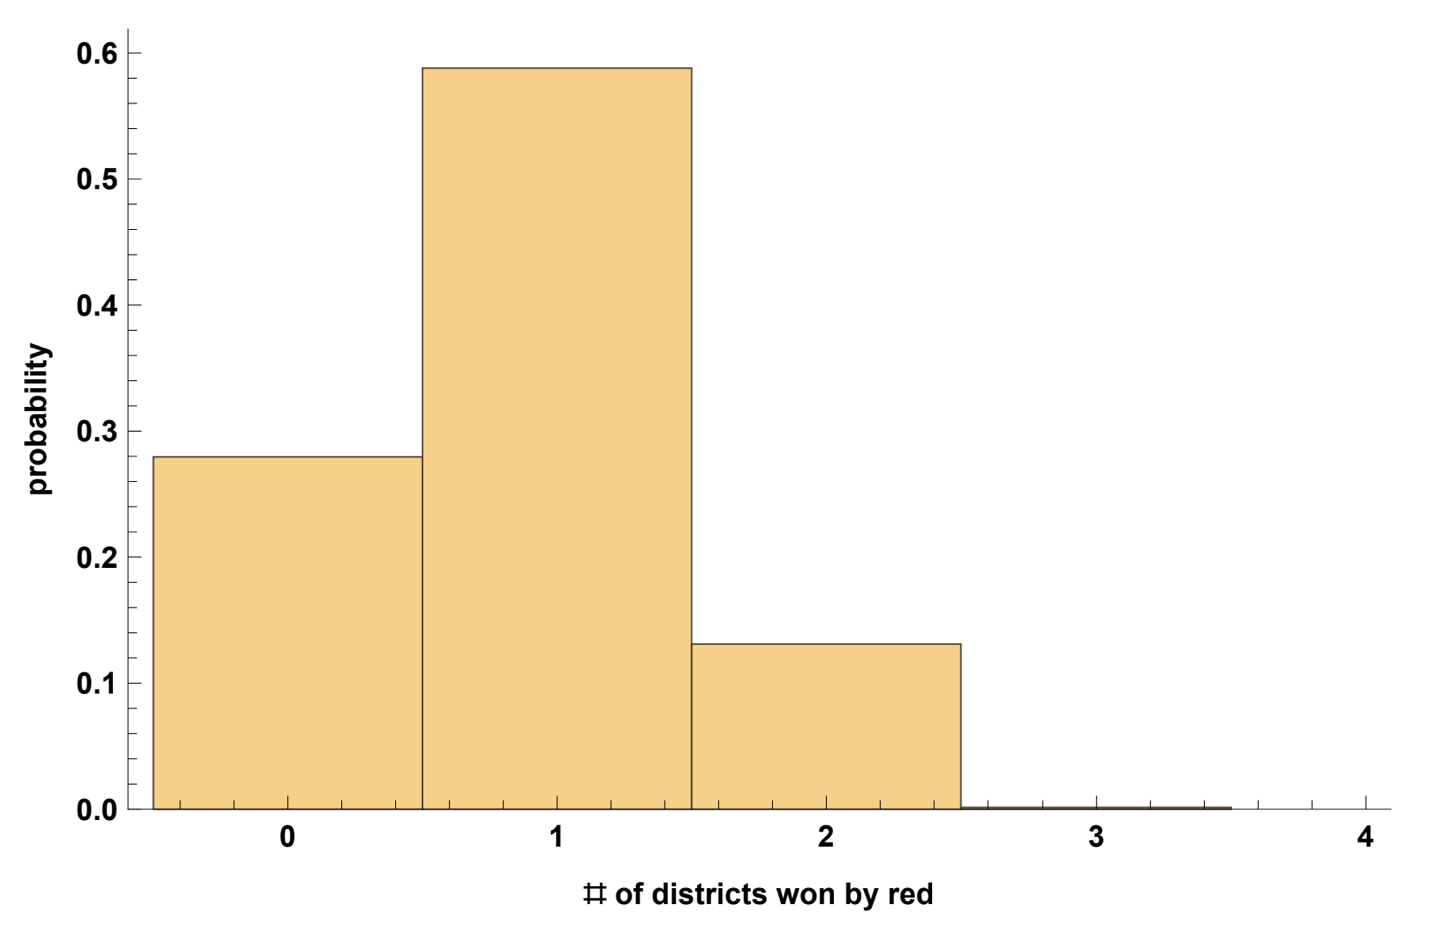
\includegraphics[scale=0.45]{random}
    \caption{North Squarolina, Random Districts}
    \label{fig:ns_rd}
    \end{figure}
    
According to the sample given by the Random Districts generated histogram (Figure \ref{fig:ns_rd}) for the number of voting districts won by red, neither 0, 1, nor 2 votes for red appears extremely unlikely. This model gives us almost nothing. Red seems to have a likelihood of winning 2 districts that is over 10\%, which seems high given real-life constraints.

\subsubsection{Using Random Districts of Equal Size}
Our Random Districts of Equal Size algorithm is far more accurate because it restricts districting to maps with districts of the same sizes. An example districting obtained by the ESRD algorithm is shown below (Figure \ref{fig:rdeqd}).

\begin{figure}[h!]
    \centering
    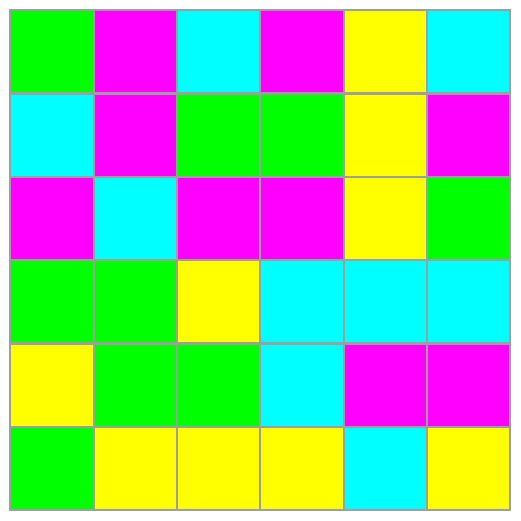
\includegraphics[scale=0.60]{rdeq_districting.pdf}
    \caption{North Squarolina, Equal-Sized Random Districts}
    \label{fig:rdeqd}
    \end{figure}
It is, however, not ideal because it still generates mostly noncontiguous (and therefore unrealistic) districting schemes. 
    \begin{figure}[h!]
    \centering
    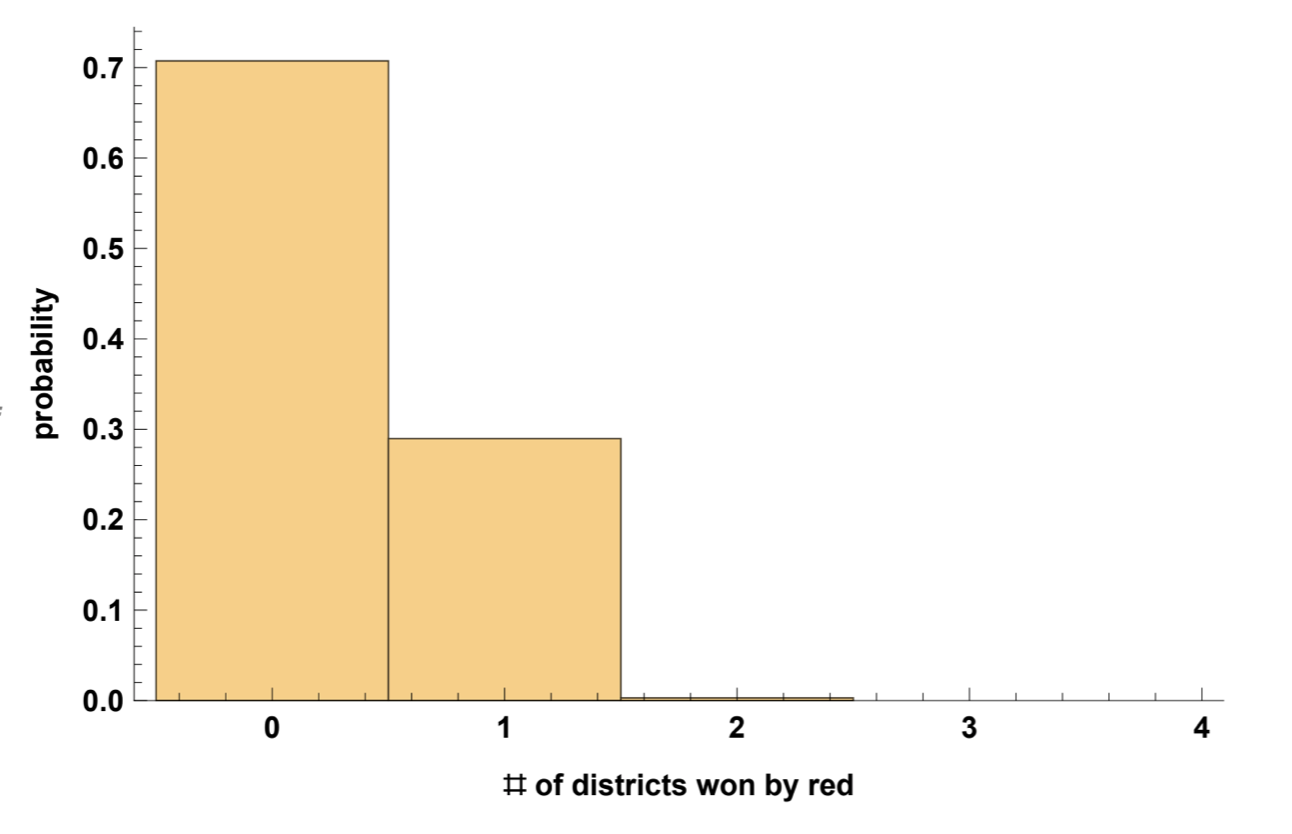
\includegraphics[scale=0.5]{random_equal}
    \caption{North Squarolina, Equal-Sized Random Districts Size Histogram}
    \label{fig:random_equal}
    \end{figure}
Out of the $100000$ districtings we generated with random districts of equal size, only a few hundred managed to win 2 districts for red. According to this sample given by the Random Districts of Equal Size generated histogram the probability of red winning is 0.00296 (around 3 in 1000). This appears to suggest that voting patterns that give red 2 districts are extremely unlikely and that districting scheme (C) is Gerrymandered.

\subsubsection{Using MCMC Contiguous Districts}
The MCMC generated districts are contiguous, and so they could be valid as real voting districts. Figure \ref{fig:mcmc_district} shows a random MCMC generated districting.
\par In Figure \ref{fig:MCMC}, we see that contiguous districts are more likely to give a seat to red than the less realistic non-contiguous random districts. Using this histogram, we can see that districting (C) still produces an extremely unlikely election outcome--reinforcing our belief that discricting (C) is probably the result of gerrymandering.

    \begin{figure}[h!]
    \centering
    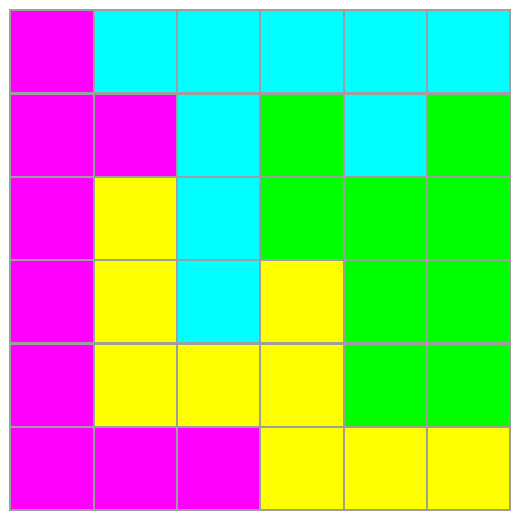
\includegraphics[scale=0.5]{mcmc_districting.pdf}
    \caption{North Squarolina, example of MCMC contiguous districts}
    \label{fig:mcmc_district}
    \end{figure}

    \begin{figure}[h!]
    \centering
    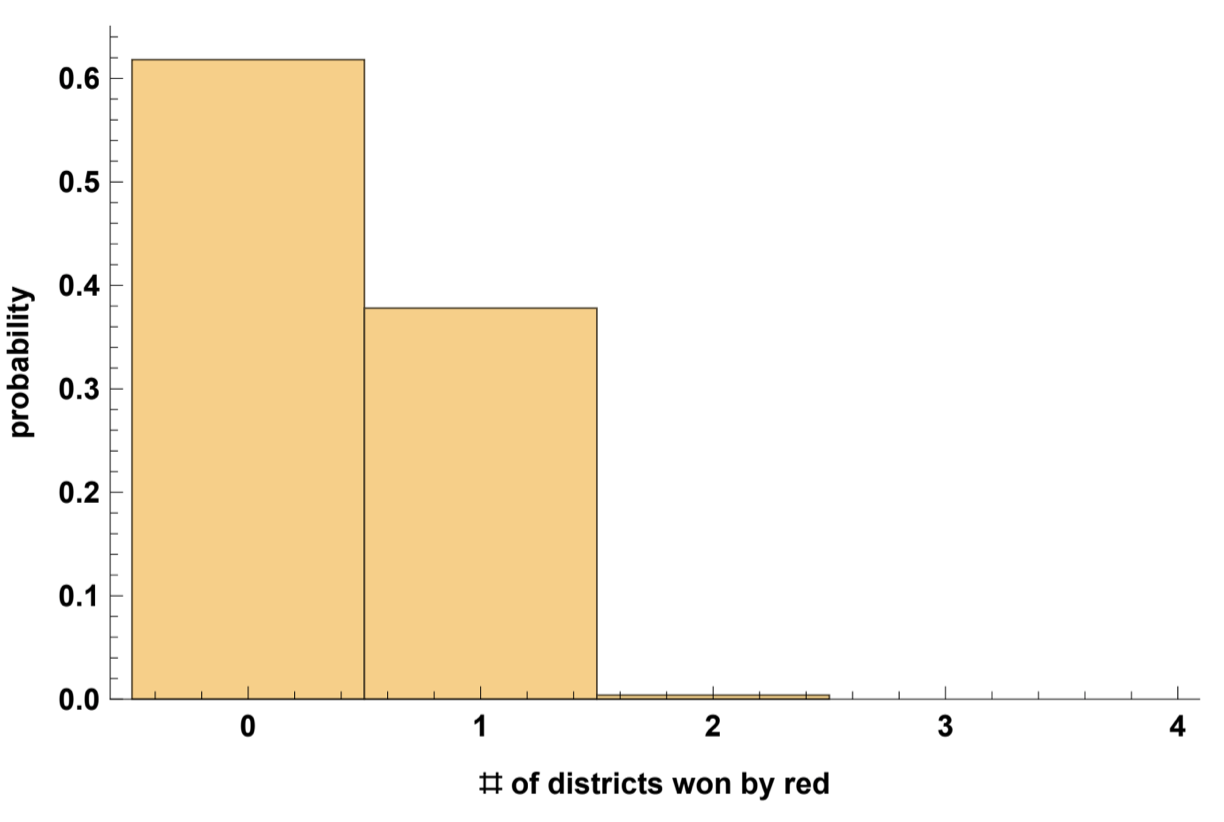
\includegraphics[scale=0.5]{MCMC}
    \caption{North Squarolina, distribution of election outcomes over random MCMC contiguous districts}
    \label{fig:MCMC}
    \end{figure}








\subsection{Is North Carolina Gerrymandered?}
Fundamentally, these algorithms burn down to methods for randomly partitioning graphs. We have been partitioning grid graphs to model North Squarolina, but we can just as easily partition any other arbitrary graph. We use North Carolina as an example.
\par We start by generating the adjacency graph for counties in North Carolina (Figure \ref{fig:nc_adj}). (See Code Appendix for details.)

    \begin{figure}[h!]
    \centering
    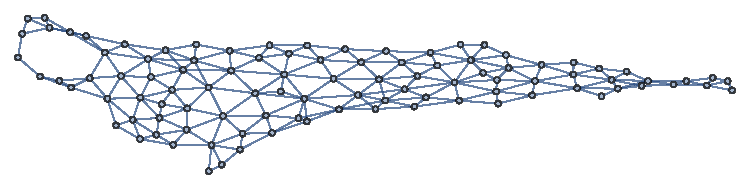
\includegraphics[scale=0.7]{NC_adj_graph.pdf}
    \caption{Adjacency graph of North Carolina counties.}
    \label{fig:nc_adj}
    \end{figure}
    
\par There is a smaller unit of voting data than counties: VTDs, otherwise known as precincts. However, VTDs change between elections, and do not have fully unique identifiers, and so we cannot reliably align election results with an adjacency graph. However, we can abstract VTD level data to county level data, and perform the data alignment over counties very easily. We do this with voting data from OpenElections \cite{openelections}.

    \begin{figure}[h!]
    \centering
    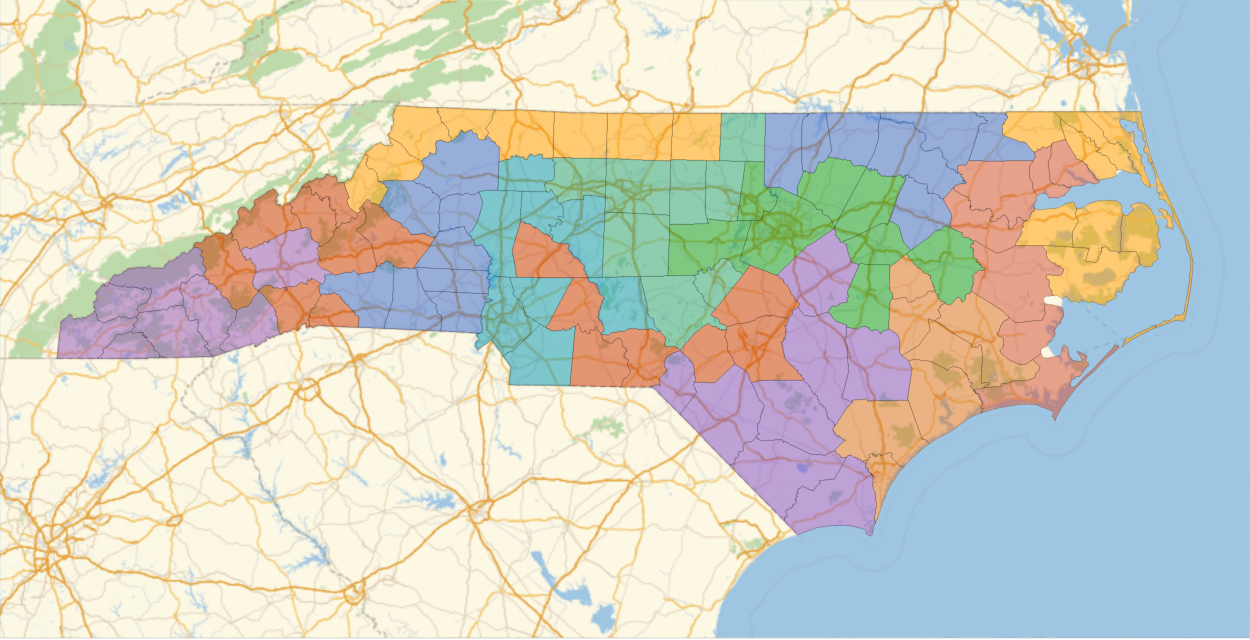
\includegraphics[scale=0.5]{nc_random_districting.pdf}
    \caption{A random districting of North Carolina.}
    \label{fig:nc_random_districting}
    \end{figure}

\par In Figure \ref{fig:nc_random_districting}, we generate a random redistricting by applying our MCMC algorithm to the county graph. As before, we can create a large number of random districtings and see how many districts each party is expected to win. Figure \ref{fig:nc_dist} shows the distribution of the number random districts that would be won by republicans. Our voting data is from 2012, when 9 of the 13 congressional districts on North Carolina were won by republicans. Our random districtings show that this is the most likely outcome, regardless of Gerrymandering.

    \begin{figure}[h!]
    \centering
    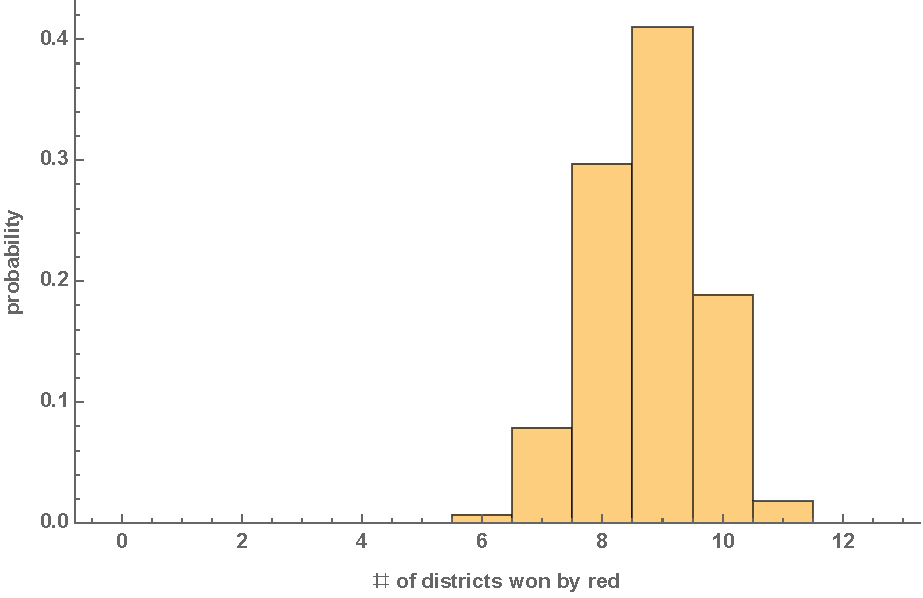
\includegraphics[scale=0.7]{nc_dist.pdf}
    \caption{Distribution of the number of districts won by republicans in $10000$ random districtings of North Carolina.}
    \label{fig:nc_dist}
    \end{figure}

\subsection{Potential Impact of Gerrymandering}
Using the model we have developed, we can also assess the potential impact of Gerrymandering for a given voter arrangement. Algorithm \ref{alg:esrd} can be modified to generate random voter arrangements by substituting $V$ for $D$ in the procedure, substituting a set of party voting differences ${-1, 1}$ for $L$ and omitting the part about recording voter outcomes, yields a randomly generated voter arrangement. This can be modified so that each party wins a a specified fraction of the total number of voting blocks. See the Code Appendix for further information. The MCMC algorithm can be applied to all these random voter arrangements to assess the average number of voters won and the maximum number of possible voters won by a given party using a highly biased districting. The results of the procedure are below, applied to North Squarolina.

    \begin{figure}[h!]
    \centering
    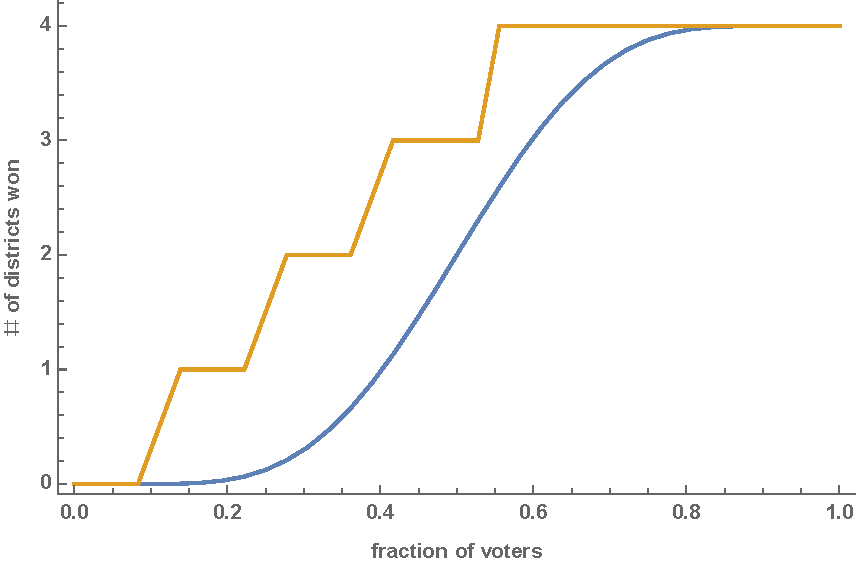
\includegraphics[scale=0.7]{b.pdf}
    \caption{Seats Won vs. Fraction of Voters Won}
    \label{fig:cdf}
    \end{figure}
\par
Plotted in Figure \ref{fig:cdf} are both the average values for the fraction of voters by party A and the maximum number of districts that could possible won by party A depending on the districting. In other words, the gold line shows the extreme-case possibility of Gerrymandering in A's favor, whereas the blue line shows the average votes won by A across the the random possible districtings generated by Algorithm \ref{alg:mcmc}. As expected, at extremely low values of vote-getting for A, Gerrymandering can't assure that A will obtain any seats. At extremely high values of A, Gerrymandering in A's won't yields more seats than average because the average number of seats won by A is the maximum number of seats won by A. (That said, it would be worth it to explore how Gerrymandering can improve Party A's confidence in securing those seats). 
\par
We can also apply this calculation to visualize how specific proposals deviate from the average number of seats won for a given voting arrangement. Applying this to the districting proposals and the voter arrangement in North Squarolina, we obtain Figure \ref{fig:cdf_fancy}.


    \begin{figure}[h!]
    \centering
    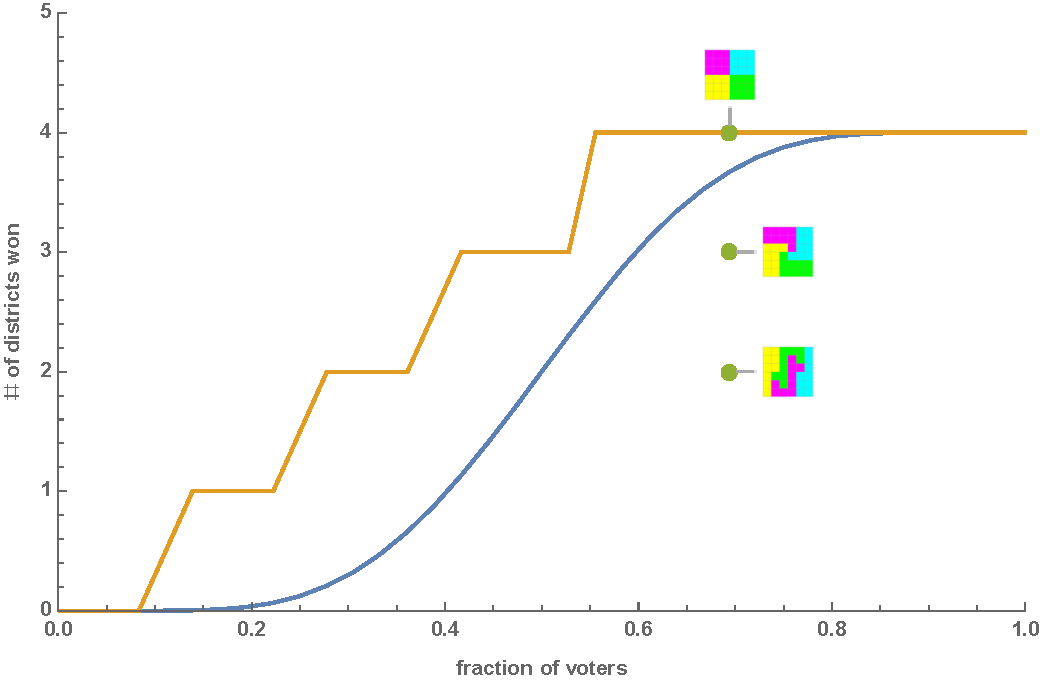
\includegraphics[scale=0.7]{c.pdf}
    \caption{Seats Won vs. Fraction of Voters Won - Depicts Proposals}
    \label{fig:cdf_fancy}
    \end{figure}
\section{Strengths and Weaknesses}

\begin{itemize}
    \item  Our Markov Chain Monte Carlo Method may not generate a good enough attempt at a perfectly random set of samples--our approximation may be flawed. Although the chain appears to eventually ``flatten out'' and distribute the probability of being in any district uniformly across all blocks, it may still unfairly favor some districting patterns over others. For example, our construction of our Markov Chain may be biased towards taking certain types of districting patterns over others--we can guess that it's not, but the truth is that we don't know. Maybe an outlier that occurs with 0.001 frequency in our MCMC sample--and looks like Gerrymandering--but it actually occurs with 0.01 frequency (a much less convincing number) in real life because it's a strange case that's hard for the chain to reach.
  \item In our simplified model we assume unanimously voting blocks. However, our model easily generalizes to any form of voting behavior, since our random district generation is meant to be unbiased and therefore independent of voting behavior. Just like in the simplified process described in this paper, we generate our random districts with our MCMC method independently of voting behavior, and then use this generated sample to inform us of low-probability events that favor one party over the other.
  \item We assume that the people who draw district lines are able to (or at least believe they are able to) predict future voting patterns based on past patterns. Obviously, voting patters often can be predicted based on past consistency, although not quite as easily as the case in North Squarolina. And when looking for most cases of Gerrymandering, we must assume relatively consistent voting patterns, and assume it is the districting map--not the election itself--that determines most of the outcome. Sometimes this is not necessarily the case. \textit{But since the act of Gerrymandering itself is flawed by the same assumption as our model}, we don't see this as a flaw in our model. 
\end{itemize}
\subsection{Using $\sqrt{2\epsilon}$ to Bound Our Results for Mathematical Rigor}
   A recently published paper explains that as long as our Markov Chain is reversible and can reach its steady-state, it will well-approximate a random sample as given by the theorem below, which we quote verbatim from the paper \cite{CMU}:

\begin{theorem} 
Let $M = X_0 , X_1 , ...$ be a reversible Markov chain with a stationary distribution $\pi$, and suppose the states of $M$ have real-valued labels. If $X_0 \sim \pi$, then for any fixed $k$, the probability that the label of $X_0$ is an $\epsilon-outlier$ from among the list of labels observed in the trajectory
$X_0 , X_1 , X_2 , ... , X_k$ is at most $\sqrt{2\epsilon}$.
\end{theorem}

In our justification for the Markov Chain Markov Carlo method as a good approximation for randomness we talk about how the chain flattens out into grey and begins to well-approximate a seemingly random sample, since the probability of any voting block being in any district, given $n$ districts, gets closer and closer to $1/n$ as we take our chain further and further. This may not indicate a perfect approximation of randomness, but this does signal that our chain is consistently bouncing around all over and reaching what appears to be a dynamic steady state. Since we can see strong evidence of our chain reaching a dynamic steady state--we know for certain that it will eventually reach the state after a certain number of iterations--and we know that the probability of reaching any specific districting scheme with regions of equal size using our model is $>0$, it then holds that we can use the theorem to more rigorously quantify outliers.

If, when using the sample for North Squarolina generated from MCMC Contiguous Districts given by the histogram in the last section, we find 189 out of 100k samples where red win two districts, this would seem to indicate that the probability of red winning 2 districts is $0.00189$. Using the much more mathematically rigorous bound given by the theorem above, however, we can find that the upper bound for the true probability is $\sqrt{2\times0.00189} = 0.0615$, which is much higher than our actual result. Although we can believe that the probability that red wins two districts is almost definitely less than one half of one percent, we can only say with practical certainty that the probability is less than about 6\%. In this example, North Squarolina is small enough where the the percentage produced by this rigorous bound is too large to mean anything of much significance, but applying our model to larger regions will yield small and inarguable upper bounds. Studies we read that used applied similar MCMC methods on larger areas such as states generated probabilities of $1\times10^-8$ or smaller, which are small enough estimations generate a significantly small, mathematically defensible upper bound for the probability of an event happening. Many times we are able to say with practical certainty that the probability of creating a system that randomly favors one party over the other cannot be greater than 1 in 1000, which would be clear and nearly irrefutable evidence of gerrymandering.

\section{Comparing Our Model to the Efficiency Gap}
\subsection{Defining the Efficiency Gap Method}
    The efficiency gap is a metric that tries to quantify the partisan bias of a districting scheme based on historical data. To arrive at this model, we begin by considering a districting scheme with partisan bias to be one in which the d of one party are disproportionately "wasted." That is, the seats won per vote are smaller for one party than for the other. In a given district, given that party A secures \(a\) votes and party B secures \(b\) votes, we calculate the pair of values \((w_a, w_b)\) to respectively be number of votes wasted by party A and number of votes wasted by party V. We can compute these values with the function \(w(a,b )\):
    \[
        w(a,b)= (w_a, w_b) = \begin{cases}
        (a-(\floor{\frac{a+b}{2}}+1), b) & a\geq b\\
        (a, a-(\floor{\frac{a+b}{2}}+1)) & b < a
        \end{cases}
    \]
    \par
    If party A loses a district (if \(a<b\)), then all \(a\) of its votes are wasted in that district. But in the case that party A wins the district, then the number of wasted votes is the difference between votes for A and the votes that A needed to win the district. The number of votes needed to win the district is equal to the floor of the total number of votes plus one. For instance, in a district where 100 people voted between party A and party B, the total votes are obtained through \(a+b=100\), and the number of votes either party needs to win is \(\floor{\frac{100}{2}}+1=50+1=51\).
    \par
    Examining an entire state composed of several districts, then \((a,b)\) represents individual districts in the space of all districts \(d\). Examining the entire state, the efficiency gap in favor of party A is defined to be the difference between B's wasted votes and A's wasted votes across every district, weighted by the inverse of the total number of votes:
    
    \[e_b(w_1, w_2) = \frac{\sum_{(a,b)\in d}{w_b-w_a}}{\sum_{(a,b)\in d}{a+b}}\]
    
    The efficiency gap in favor of party B is the negative of the efficiency gap in favor of party A. This formula measures the difference between votes wasted by party A and party B, then normalizes the difference by dividing by total votes.
    
    
    
\subsection{Why the Efficiency Gap is Not Enough}
The efficiency gap is simply an evaluation of how districting favors one party over another. By counting the difference in wasted votes divided by total votes it counts the ``losses'' incurred by the unfavored party. However, without any acknowledgement of probability the efficiency gap is not useful as an indicator for Gerrymandering--naturally, given a certain voting arrangement, it might be more likely that one party gets favored over the other. For example, in the case where 30\% of voters favor one party, but they are scattered uniformly about the other 70\%, most districtings will largely favor the majority party because most districtings will contain around a 70\% to 30\% balance in each district. However, the resulting efficiency gap of 10\% would, to an efficiency gap believer, seem to scream bloody murder. \textit{Absolutely nothing abnormal happened in the drawing of the districts,} and yet according to the efficiency gap metric we have a case of Gerrymandering. Any state with an efficiency gap of $>7\%$ has been condemned in the news.

\section{Conclusion}
A probability-driven approach is essential to quantifying gerrymandering in a court of law. A metric like efficiency gap can often be the result of a coincidence such as obvious geographical boundaries or something like the example outlined above, as opposed to actual gerrymandering. With our approach, defining situations that favor one party over the other in terms of probability, we can define gerrymandering as a very low probability event that favors one party over the other. If we find an action that favors one party over the other with very low probability, we most likely found an action that favors one party over the other deliberately, and deliberately favoring one party over the other is Gerrymandering by definition.

\newpage
\begin{thebibliography}

\bibitem{CLLI}
“Gerrymander.” \textit{LII / Legal Information Institute}, Cornell University Law School, www.law.cornell.edu/wex/Gerrymander.

\bibitem{psmag} 
Jacobs, Tom. \textit{“The Policy Consequences of Partisan Gerrymandering.”} Pacific Standard, Pacific Standard, 4 Oct. 2017, psmag.com/news/the-policy-consequences-of-partisan-gerrymandering.

\bibitem{problem}
Brown Division of Applied Math. \textit{Brown Mathematical Contest for Modeling 2018 Problems}. Brown Mathematical Contest for Modeling 2018 Problems, 2018.

\bibitem{GW}
“Gill v. Whitford.” \textit{Wikipedia}, Wikimedia Foundation, 7 Aug. 2018, en.wikipedia.org/wiki/Gill_v._Whitford.

\bibitem{openelections}
“Home | OpenElections: Certified Election Results. For Everyone.” \textit{Home | OpenElections: Certified Election Results. For Everyone.}, www.openelections.net/.

\bibitem{Harv}
Fifield, Benjamin, et al. \textit{A New Automated Redistricting Simulator Using Markov Chain Monte Carlo.}, https://imai.fas.harvard.edu/research/files/redist.pdf

\bibitem{CMU}
https://www.cmu.edu/news/stories/archives/2018/january/images/MATH-18-114_Math\%20Newsletter\_Gerrymandering.pdf

\end{thebibliography}

\section{Code Appendix}

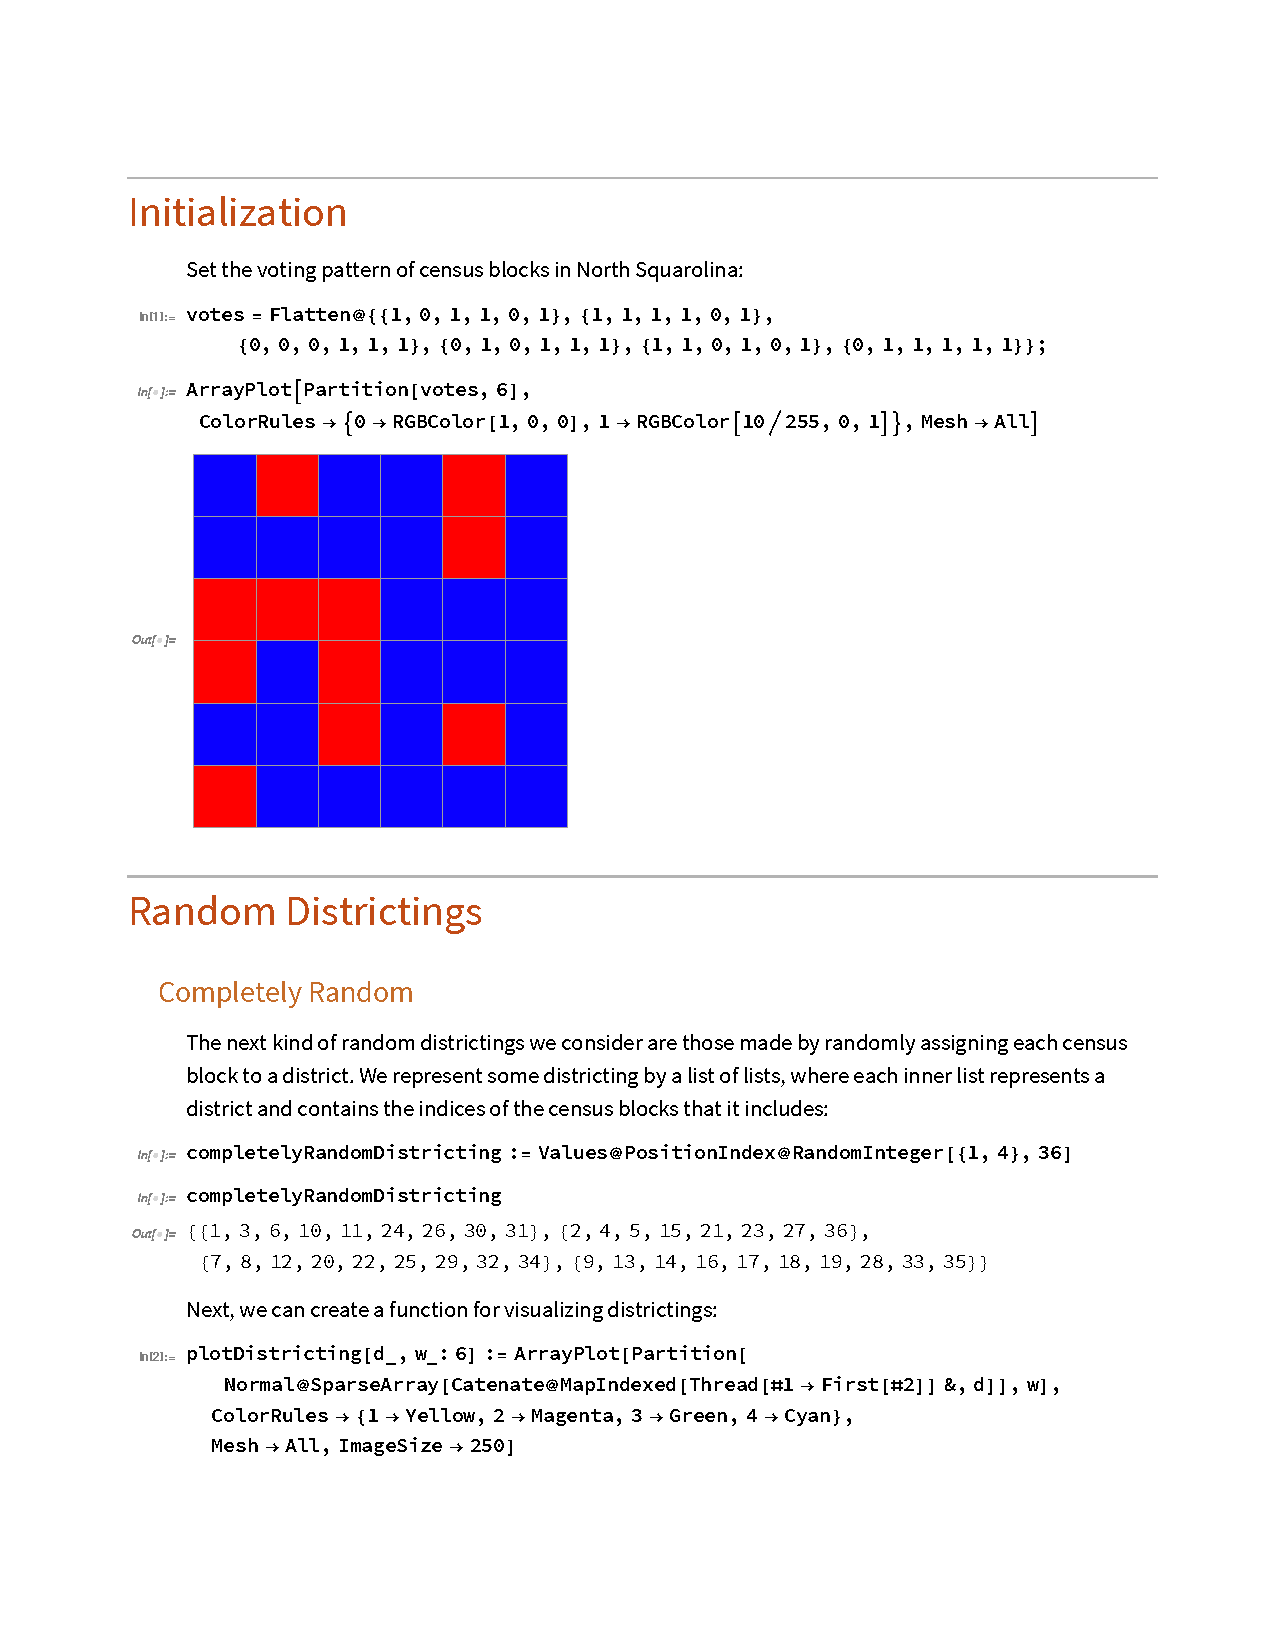
\includepdf[pages=1-14]{codeAppendix.pdf}

\end{document}
